% Gauss reduction: the basis b1=(2.7,2.5), b2=(3.4,4.4) (red) and the reduced basis (1.3,-1.3), (0.7,1.9) of the same lattice (green).
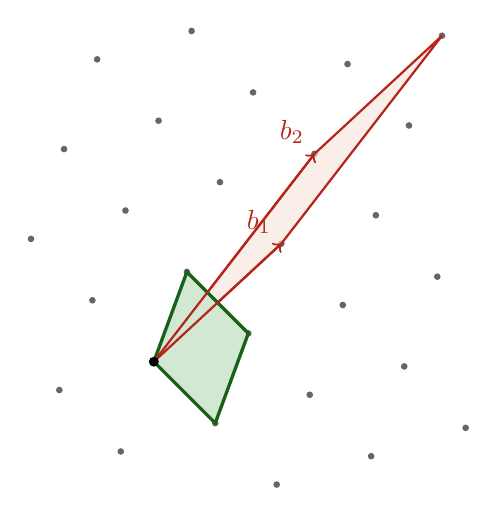
\begin{tikzpicture}[scale=0.6]
\fill[black!60] (-2.6000,2.6000) circle (2pt);
\fill[black!60] (-1.9000,4.5000) circle (2pt);
\fill[black!60] (-1.2000,6.4000) circle (2pt);
\fill[black!60] (-2.0000,-0.6000) circle (2pt);
\fill[black!60] (-1.3000,1.3000) circle (2pt);
\fill[black!60] (-0.6000,3.2000) circle (2pt);
\fill[black!60] (0.1000,5.1000) circle (2pt);
\fill[black!60] (0.8000,7.0000) circle (2pt);
\fill[black!60] (-0.7000,-1.9000) circle (2pt);
\fill[black!60] (0.0000,0.0000) circle (2pt);
\fill[black!60] (0.7000,1.9000) circle (2pt);
\fill[black!60] (1.4000,3.8000) circle (2pt);
\fill[black!60] (2.1000,5.7000) circle (2pt);
\fill[black!60] (1.3000,-1.3000) circle (2pt);
\fill[black!60] (2.0000,0.6000) circle (2pt);
\fill[black!60] (2.7000,2.5000) circle (2pt);
\fill[black!60] (3.4000,4.4000) circle (2pt);
\fill[black!60] (4.1000,6.3000) circle (2pt);
\fill[black!60] (2.6000,-2.6000) circle (2pt);
\fill[black!60] (3.3000,-0.7000) circle (2pt);
\fill[black!60] (4.0000,1.2000) circle (2pt);
\fill[black!60] (4.7000,3.1000) circle (2pt);
\fill[black!60] (5.4000,5.0000) circle (2pt);
\fill[black!60] (6.1000,6.9000) circle (2pt);
\fill[black!60] (4.6000,-2.0000) circle (2pt);
\fill[black!60] (5.3000,-0.1000) circle (2pt);
\fill[black!60] (6.0000,1.8000) circle (2pt);
\fill[black!60] (6.6000,-1.4000) circle (2pt);
\draw[BrickRed,thick,fill=BrickRed!10,fill opacity=0.6] (0,0) -- (2.7000,2.5000) -- (6.1000,6.9000) -- (3.4000,4.4000) -- cycle;
\draw[ForestGreen!70!black,very thick,fill=ForestGreen!20] (0,0) -- (1.3000,-1.3000) -- (2.0000,0.6000) -- (0.7000,1.9000) -- cycle;
\draw[->,BrickRed,thick] (0,0) -- (2.7000,2.5000) node[above left] {$b_1$};
\draw[->,BrickRed,thick] (0,0) -- (3.4000,4.4000) node[above left] {$b_2$};
\fill (0,0) circle (3pt);
\end{tikzpicture}
